%
\normalsize%
\subsection{ValueSpecification}%
\label{sec:uml:ValueSpecification}%
A \uml{ValueSpecification} is the specification of a (possibly empty) set of values. See UML 2.5.1 specification section 8.%
\newline%
\linebreak%


\begin{figure}[h!]%
\centering%
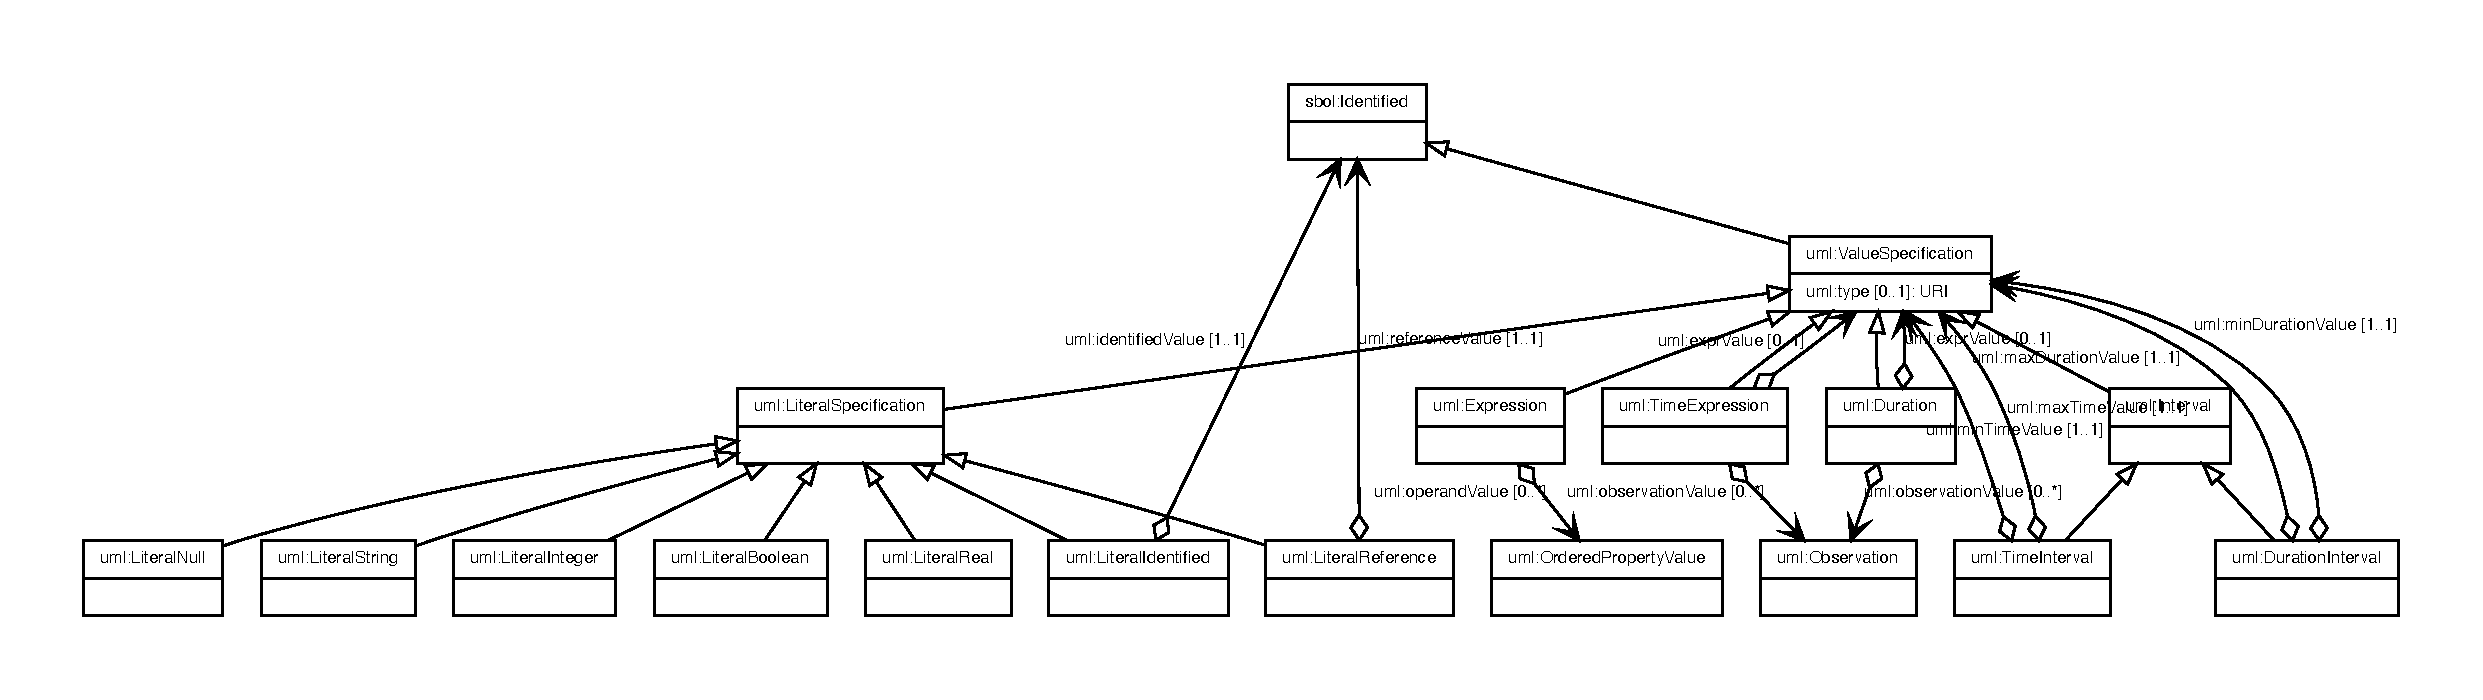
\includegraphics[width=1.0\textwidth]{uml_classes/ValueSpecification_abstraction_hierarchy.pdf}%
\caption{ValueSpecification}%
\label{fig:ValueSpecification}%
\end{figure}

%
The \uml{ValueSpecification} class is shown in \ref{fig:ValueSpecification}. It is derived from \sbol{Identified} and includes the following specializations: \uml{LiteralSpecification}, \uml{Expression}, \uml{TimeExpression}, \uml{Duration}, \uml{Interval}. %
This class includes the following properties: \uml{type}. %
\begin{itemize}%
\item%
The \uml{type} property is OPTIONAL and has a singleton value of type URISpecifies a set of Type instances constraining the allowed values. See UML 2.5.1 specification section 7.5.%
\end{itemize}%
\subsubsection{LiteralSpecification}%
\label{sec:uml:LiteralSpecification}%
A \uml{LiteralSpecification} identifies a literal constant being modeled. See UML 2.5.1 specification section 8.2.%
\newline%
\linebreak%
The \uml{LiteralSpecification} class is shown in \ref{fig:ValueSpecification}. It is derived from \uml{ValueSpecification} and includes the following specializations: \uml{LiteralNull}, \uml{LiteralString}, \uml{LiteralInteger}, \uml{LiteralBoolean}, \uml{LiteralReal}, \uml{LiteralIdentified}, \uml{LiteralReference}. %
%
\paragraph{LiteralNull}%
\label{sec:uml:LiteralNull}%
A \uml{LiteralNull} specifies the lack of a value. See UML 2.5.1 specification section 8.2.%
\newline%
\linebreak%
The \uml{LiteralNull} class is shown in \ref{fig:ValueSpecification}. It is derived from \uml{LiteralSpecification}.%
%
\paragraph{LiteralString}%
\label{sec:uml:LiteralString}%
A \uml{LiteralSpecification} identifies a literal constant being modeled. See UML 2.5.1 specification section 8.2.%
\newline%
\linebreak%
The \uml{LiteralString} class is shown in \ref{fig:ValueSpecification}. It is derived from \uml{LiteralSpecification}.%
This class includes the following properties: \uml{stringValue}. %
\begin{itemize}%
\item%
The \uml{stringValue} property is REQUIRED and has a singleton value of type stringThe specified String value.%
\end{itemize}%
\paragraph{LiteralInteger}%
\label{sec:uml:LiteralInteger}%
A \uml{LiteralInteger} is a specification of an Integer value. See UML 2.5.1 specification section 8.2.%
\newline%
\linebreak%
The \uml{LiteralInteger} class is shown in \ref{fig:ValueSpecification}. It is derived from \uml{LiteralSpecification}.%
This class includes the following properties: \uml{integerValue}. %
\begin{itemize}%
\item%
The \uml{integerValue} property is REQUIRED and has a singleton value of type integerThe specified Integer value.%
\end{itemize}%
\paragraph{LiteralBoolean}%
\label{sec:uml:LiteralBoolean}%
A \uml{LiteralBoolean} is a specification of a Boolean value. See UML 2.5.1 specification section 8.2.%
\newline%
\linebreak%
The \uml{LiteralBoolean} class is shown in \ref{fig:ValueSpecification}. It is derived from \uml{LiteralSpecification}.%
This class includes the following properties: \uml{booleanValue}. %
\begin{itemize}%
\item%
The \uml{booleanValue} property is REQUIRED and has a singleton value of type booleanThe specified Boolean value.%
\end{itemize}%
\paragraph{LiteralReal}%
\label{sec:uml:LiteralReal}%
A \uml{LiteralReal} is a specification of a Real value. See UML 2.5.1 specification section 8.2.%
\newline%
\linebreak%
The \uml{LiteralReal} class is shown in \ref{fig:ValueSpecification}. It is derived from \uml{LiteralSpecification}.%
This class includes the following properties: \uml{realValue}. %
\begin{itemize}%
\item%
The \uml{realValue} property is REQUIRED and has a singleton value of type floatThe specified Real value.%
\end{itemize}%
\paragraph{LiteralIdentified}%
\label{sec:uml:LiteralIdentified}%
A \uml{LiteralIdentified} is used for linking SBOL objects as a child object to UML objects.%
\newline%
\linebreak%
The \uml{LiteralIdentified} class is shown in \ref{fig:ValueSpecification}. It is derived from \uml{LiteralSpecification}.%
This class includes the following properties: \uml{identifiedValue}. %
\begin{itemize}%
\item%
The \uml{identifiedValue} property is REQUIRED and contains a URI reference to an associated object of type IdentifiedThe embedded SBOL object%
\end{itemize}%
\paragraph{LiteralReference}%
\label{sec:uml:LiteralReference}%
A \uml{LiteralReference} is used for embedding SBOL objects as a reference.%
\newline%
\linebreak%
The \uml{LiteralReference} class is shown in \ref{fig:ValueSpecification}. It is derived from \uml{LiteralSpecification}.%
This class includes the following properties: \uml{referenceValue}. %
\begin{itemize}%
\item%
The \uml{referenceValue} property is REQUIRED and contains a URI reference to an associated object of type IdentifiedThe referenced SBOL object.%
\end{itemize}%
\subsubsection{Expression}%
\label{sec:uml:Expression}%
An \uml{Expression} represents a node in an expression tree, which may be non-terminal or terminal. It defines a symbol, and has a possibly empty sequence of operands that are ValueSpecifications. See UML 2.5.1 specification section 8.6.5.1.%
\newline%
\linebreak%
The \uml{Expression} class is shown in \ref{fig:ValueSpecification}. It is derived from \uml{ValueSpecification}.%
This class includes the following properties: \uml{isOrdered}, \uml{symbolValue}, \uml{operandValue}. %
\begin{itemize}%
\item%
The \uml{operandValue} property is OPTIONAL and contains URI references to associated objects of type OrderedPropertyValueSpecifies a sequence of operand ValueSpecifications.%
\item%
The \uml{isOrdered} property is REQUIRED and has a singleton value of type booleanFor MultiplicityElement abstract class; UML 2.5.1 specification section 7.5%
\item%
The \uml{symbolValue} property is OPTIONAL and has a singleton value of type stringThe symbol associated with this node in the expression tree.%
\end{itemize}%
\subsubsection{TimeExpression}%
\label{sec:uml:TimeExpression}%
A \uml{TimeExpression} is a \uml{ValueSpecification} that represents a time value.%
\newline%
\linebreak%
The \uml{TimeExpression} class is shown in \ref{fig:ValueSpecification}. It is derived from \uml{ValueSpecification}.%
This class includes the following properties: \uml{observationValue}, \uml{exprValue}. %
\begin{itemize}%
\item%
The \uml{observationValue} property is OPTIONAL and contains URI references to associated objects of type ObservationRefers to the Observations that are involved in the computation of the Duration value.%
\item%
The \uml{exprValue} property is OPTIONAL and contains a URI reference to an associated object of type ValueSpecificationA ValueSpecification that evaluates to the value of the Duration.%
\end{itemize}%
\subsubsection{Duration}%
\label{sec:uml:Duration}%
A \uml{Duration} is a \uml{ValueSpecification} that specifies the temporal distance between two time instants.%
\newline%
\linebreak%
The \uml{Duration} class is shown in \ref{fig:ValueSpecification}. It is derived from \uml{ValueSpecification}.%
This class includes the following properties: \uml{observationValue}, \uml{exprValue}. %
\begin{itemize}%
\item%
The \uml{observationValue} property is OPTIONAL and contains URI references to associated objects of type ObservationRefers to the Observations that are involved in the computation of the Duration value.%
\item%
The \uml{exprValue} property is OPTIONAL and contains a URI reference to an associated object of type ValueSpecificationA ValueSpecification that evaluates to the value of the Duration.%
\end{itemize}%
\subsubsection{Interval}%
\label{sec:uml:Interval}%
An \uml{Interval} defines the range between two ValueSpecifications.%
\newline%
\linebreak%
The \uml{Interval} class is shown in \ref{fig:ValueSpecification}. It is derived from \uml{ValueSpecification} and includes the following specializations: \uml{TimeInterval}, \uml{DurationInterval}. %
%
\paragraph{TimeInterval}%
\label{sec:uml:TimeInterval}%
A \uml{TimeInterval} defines the range between two TimeExpressions.%
\newline%
\linebreak%
The \uml{TimeInterval} class is shown in \ref{fig:ValueSpecification}. It is derived from \uml{Interval}.%
This class includes the following properties: \uml{minTimeValue}, \uml{maxTimeValue}. %
\begin{itemize}%
\item%
The \uml{minTimeValue} property is REQUIRED and contains a URI reference to an associated object of type ValueSpecificationRefers to the TimeExpression denoting the minimum value of the range.%
\item%
The \uml{maxTimeValue} property is REQUIRED and contains a URI reference to an associated object of type ValueSpecificationRefers to the TimeExpression denoting the maximum value of the range.%
\end{itemize}%
\paragraph{DurationInterval}%
\label{sec:uml:DurationInterval}%
A \uml{DurationInterval} defines the range between two Durations.%
\newline%
\linebreak%
The \uml{DurationInterval} class is shown in \ref{fig:ValueSpecification}. It is derived from \uml{Interval}.%
This class includes the following properties: \uml{minDurationValue}, \uml{maxDurationValue}. %
\begin{itemize}%
\item%
The \uml{minDurationValue} property is REQUIRED and contains a URI reference to an associated object of type ValueSpecificationRefers to the Duration denoting the minimum value of the range.%
\item%
The \uml{maxDurationValue} property is REQUIRED and contains a URI reference to an associated object of type ValueSpecificationRefers to the Duration denoting the maximum value of the range.%
\end{itemize}%
\subsection{Observation}%
\label{sec:uml:Observation}%
Observation specifies a value determined by observing an event or events that occur relative to other model entities.%
\newline%
\linebreak%


\begin{figure}[h!]%
\centering%
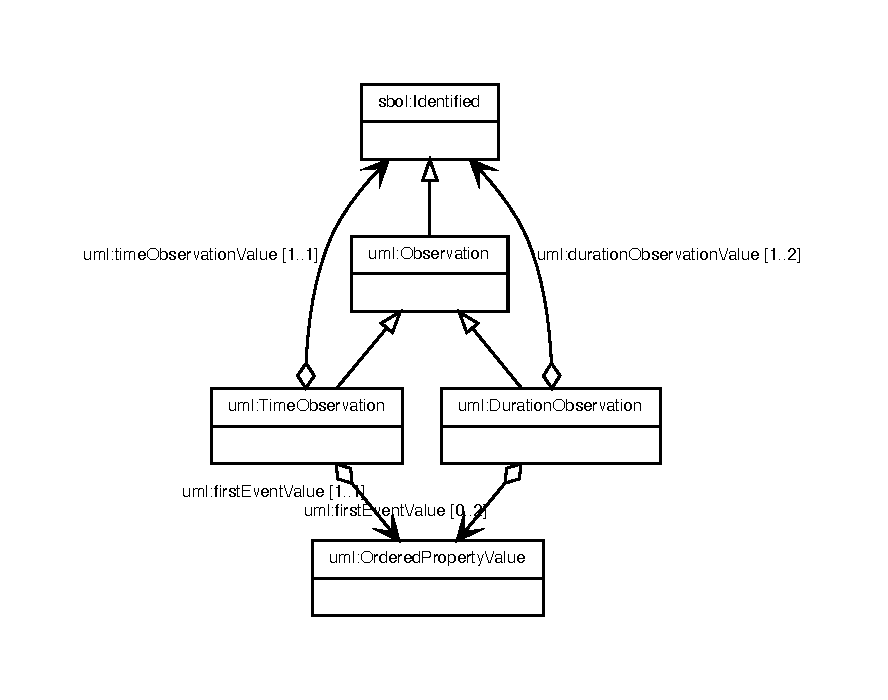
\includegraphics[width=0.634468085106383\textwidth]{uml_classes/Observation_abstraction_hierarchy.pdf}%
\caption{Observation}%
\label{fig:Observation}%
\end{figure}

%
The \uml{Observation} class is shown in \ref{fig:Observation}. It is derived from \sbol{Identified} and includes the following specializations: \uml{TimeObservation}, \uml{DurationObservation}. %
%
\subsubsection{TimeObservation}%
\label{sec:uml:TimeObservation}%
A \uml{TimeObservation} is a reference to a time instant during an execution. It points out which entity in the model to observe and whether the observation is when this entity is entered or when it is exited.%
\newline%
\linebreak%
The \uml{TimeObservation} class is shown in \ref{fig:Observation}. It is derived from \uml{Observation}.%
This class includes the following properties: \uml{timeObservationValue}, \uml{firstEventValue}. %
\begin{itemize}%
\item%
The \uml{timeObservationValue} property is REQUIRED and contains a URI reference to an associated object of type IdentifiedThe TimeObservation is determined by the entering or exiting of the event during execution.%
\item%
The \uml{firstEventValue} property is REQUIRED and contains a URI reference to an associated object of type OrderedPropertyValueThe value of firstEvent[i] is related to event[i] (where i is 1 or 2). If firstEvent[i] is true, then the correspondingobservation event is the first time instant the execution enters event[i]. If firstEvent[i] is false, then the corresponding observation event is the time instant the execution exits event[i].%
\end{itemize}%
\subsubsection{DurationObservation}%
\label{sec:uml:DurationObservation}%
A \uml{DurationObservation} is a reference to a duration during an execution. It points out the entities in the model to observe and whether the observations are when these entities are entered or exited.%
\newline%
\linebreak%
The \uml{DurationObservation} class is shown in \ref{fig:Observation}. It is derived from \uml{Observation}.%
This class includes the following properties: \uml{durationObservationValue}, \uml{firstEventValue}. %
\begin{itemize}%
\item%
The \uml{durationObservationValue} property is REQUIRED and contains URI references to associated objects of type IdentifiedThe DurationObservation is determined as the duration between the entering or exiting of a single event during execution, or the entering/exiting of one event and the entering/exiting of a second.%
\item%
The \uml{firstEventValue} property is OPTIONAL and contains URI references to associated objects of type OrderedPropertyValueThe value of firstEvent[i] is related to event[i] (where i is 1 or 2). If firstEvent[i] is true, then the correspondingobservation event is the first time instant the execution enters event[i]. If firstEvent[i] is false, then the corresponding observation event is the time instant the execution exits event[i].%
\end{itemize}%
\subsection{Constraint}%
\label{sec:uml:Constraint}%
A \sbol{Constraint} is a condition or restriction expressed in natural language text or in a machine readable language. See UML 2.5.1 specification section 7.6.%
\newline%
\linebreak%


\begin{figure}[h!]%
\centering%
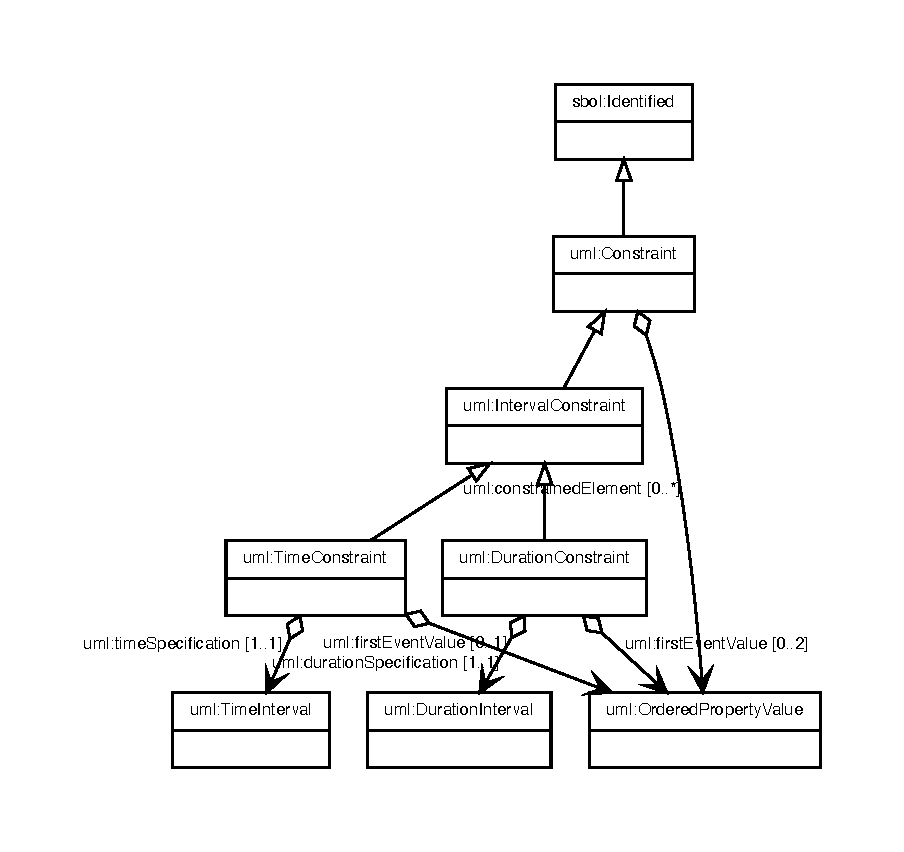
\includegraphics[width=0.7178723404255319\textwidth]{uml_classes/Constraint_abstraction_hierarchy.pdf}%
\caption{Constraint}%
\label{fig:Constraint}%
\end{figure}

%
The \uml{Constraint} class is shown in \ref{fig:Constraint}. It is derived from \sbol{Identified} and includes the following specializations: \uml{IntervalConstraint}. %
This class includes the following properties: \uml{constrainedElement}. %
\begin{itemize}%
\item%
The \uml{constrainedElement} property is OPTIONAL and contains URI references to associated objects of type OrderedPropertyValueThe OrderedPropertyValue referenced by this Constraint.%
\end{itemize}%
\subsubsection{IntervalConstraint}%
\label{sec:uml:IntervalConstraint}%
An \uml{IntervalConstraint} is a \sbol{Constraint} that is specified by an \uml{Interval}.%
\newline%
\linebreak%
The \uml{IntervalConstraint} class is shown in \ref{fig:Constraint}. It is derived from \uml{Constraint} and includes the following specializations: \uml{TimeConstraint}, \uml{DurationConstraint}. %
%
\paragraph{TimeConstraint}%
\label{sec:uml:TimeConstraint}%
A \uml{TimeConstraint} is a \sbol{Constraint} that refers to a \uml{TimeInterval}.%
\newline%
\linebreak%
The \uml{TimeConstraint} class is shown in \ref{fig:Constraint}. It is derived from \uml{IntervalConstraint}.%
This class includes the following properties: \uml{timeSpecification}, \uml{firstEventValue}. %
\begin{itemize}%
\item%
The \uml{timeSpecification} property is REQUIRED and contains a URI reference to an associated object of type TimeIntervalTheTimeInterval constraining the duration.%
\item%
The \uml{firstEventValue} property is OPTIONAL and contains a URI reference to an associated object of type OrderedPropertyValueThe value of firstEvent[i] is related to event[i] (where i is 1 or 2). If firstEvent[i] is true, then the correspondingobservation event is the first time instant the execution enters event[i]. If firstEvent[i] is false, then the corresponding observation event is the time instant the execution exits event[i].%
\end{itemize}%
\paragraph{DurationConstraint}%
\label{sec:uml:DurationConstraint}%
A \uml{DurationConstraint} is a \sbol{Constraint} that refers to a \uml{DurationInterval}.%
\newline%
\linebreak%
The \uml{DurationConstraint} class is shown in \ref{fig:Constraint}. It is derived from \uml{IntervalConstraint}.%
This class includes the following properties: \uml{durationSpecification}, \uml{firstEventValue}. %
\begin{itemize}%
\item%
The \uml{durationSpecification} property is REQUIRED and contains a URI reference to an associated object of type DurationIntervalThe DurationInterval constraining the duration.%
\item%
The \uml{firstEventValue} property is OPTIONAL and contains URI references to associated objects of type OrderedPropertyValueThe value of firstEvent[i] is related to event[i] (where i is 1 or 2). If firstEvent[i] is true, then the correspondingobservation event is the first time instant the execution enters event[i]. If firstEvent[i] is false, then the corresponding observation event is the time instant the execution exits event[i].%
\end{itemize}%
\subsection{Parameter}%
\label{sec:uml:Parameter}%
A \uml{Parameter} is a specification of an argument used to pass information into or out of an invocation of a \uml{Behavior}. See UML 2.5.1 specification section 9.4.%
\newline%
\linebreak%


\begin{figure}[h!]%
\centering%
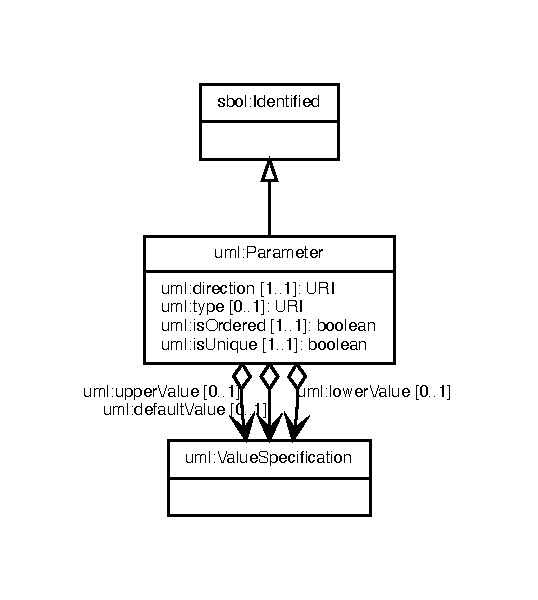
\includegraphics[width=0.3842553191489362\textwidth]{uml_classes/Parameter_abstraction_hierarchy.pdf}%
\caption{Parameter}%
\label{fig:Parameter}%
\end{figure}

%
The \uml{Parameter} class is shown in \ref{fig:Parameter}. It is derived from \sbol{Identified}.%
This class includes the following properties: \uml{direction}, \uml{type}, \uml{isOrdered}, \uml{isUnique}, \uml{upperValue}, \uml{defaultValue}, \uml{lowerValue}. %
\begin{itemize}%
\item%
The \uml{upperValue} property is OPTIONAL and contains a URI reference to an associated object of type ValueSpecificationFor MultiplicityElement abstract class; UML 2.5.1 specification section 7.5%
\item%
The \uml{defaultValue} property is OPTIONAL and contains a URI reference to an associated object of type ValueSpecificationA ValueSpecification that represents a value to be used when no argument is supplied for the Parameter.%
\item%
The \uml{lowerValue} property is OPTIONAL and contains a URI reference to an associated object of type ValueSpecificationFor MultiplicityElement abstract class; UML 2.5.1 specification section 7.5%
\item%
The \uml{direction} property is REQUIRED and has a singleton value of type URIIndicates whether a parameter is being sent into or out of a behavioral element.%
\item%
The \uml{type} property is OPTIONAL and has a singleton value of type URISpecifies a set of Type instances constraining the allowed values. See UML 2.5.1 specification section 7.5.%
\item%
The \uml{isOrdered} property is REQUIRED and has a singleton value of type booleanFor MultiplicityElement abstract class; UML 2.5.1 specification section 7.5%
\item%
The \uml{isUnique} property is REQUIRED and has a singleton value of type booleanFor MultiplicityElement abstract class; UML 2.5.1 specification section 7.5%
\end{itemize}%
\subsection{Behavior}%
\label{sec:uml:Behavior}%
Behavior is an abstract specification of how a state changes over time. This specification may be a prospective definition of a protocol or a capture of an execution trace. See UML 2.5.1 specification section 13.2.%
\newline%
\linebreak%


\begin{figure}[h!]%
\centering%
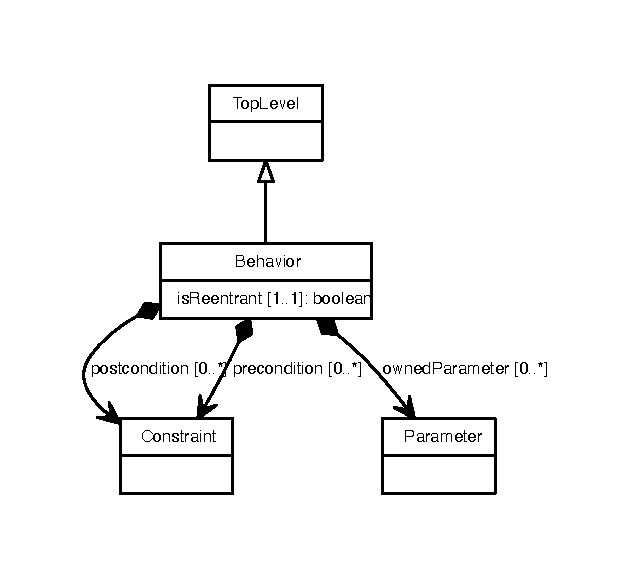
\includegraphics[width=0.6448936170212766\textwidth]{uml_classes/Behavior_abstraction_hierarchy.pdf}%
\caption{Behavior}%
\label{fig:Behavior}%
\end{figure}

%
The \uml{Behavior} class is shown in \ref{fig:Behavior}. It is derived from \sbol{TopLevel} and includes the following specializations: \uml{Activity}. %
This class includes the following properties: \uml{ownedParameter}, \uml{postcondition}, \uml{precondition}. %
\begin{itemize}%
\item%
The \uml{ownedParameter} property is OPTIONAL and contains URI references to associated objects of type OrderedPropertyValue a list of Parameters to the Behavior which describes the order and type of arguments that can be given when the Behavior is invoked and of the values which will be returned when the Behavior completes its execution.%
\item%
The \uml{postcondition} property is OPTIONAL and contains URI references to associated objects of type ConstraintAn optional set of Constraints specifying what is fulfilled after the execution of the Behavior is completed, if its precondition was fulfilled before its invocation.%
\item%
The \uml{precondition} property is OPTIONAL and contains URI references to associated objects of type ConstraintAn optional set of Constraints specifying what must be fulfilled before the Behavior is invoked.%
\end{itemize}%
\subsubsection{Activity}%
\label{sec:uml:Activity}%
An \prov{Activity} coordinates and groups steps in a protocol or workflow. See UML 2.5.1 specification section 15.%
\newline%
\linebreak%
The \uml{Activity} class is shown in \ref{fig:Behavior}. It is derived from \uml{Behavior}.%
This class includes the following properties: \uml{edge}, \uml{node}. %
\begin{itemize}%
\item%
The \uml{edge} property is OPTIONAL and contains URI references to associated objects of type ActivityEdgeActivityEdges expressing flow between the nodes of the Activity.%
\item%
The \uml{node} property is OPTIONAL and contains URI references to associated objects of type ActivityNodeActivityNodes coordinated by the Activity.%
\end{itemize}%
\subsection{OrderedPropertyValue}%
\label{sec:uml:OrderedPropertyValue}%


\begin{figure}[h!]%
\centering%
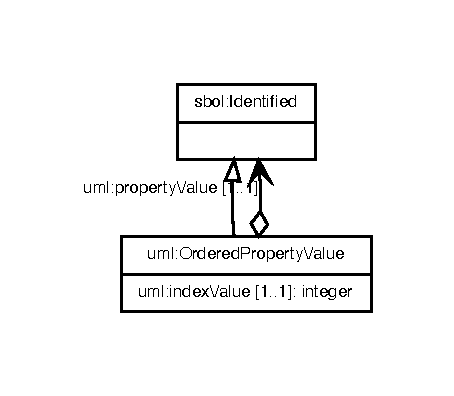
\includegraphics[width=0.32468085106382977\textwidth]{uml_classes/OrderedPropertyValue_abstraction_hierarchy.pdf}%
\caption{OrderedPropertyValue}%
\label{fig:OrderedPropertyValue}%
\end{figure}

%
The \uml{OrderedPropertyValue} class is shown in \ref{fig:OrderedPropertyValue}. It is derived from \sbol{Identified}.%
This class includes the following properties: \uml{indexValue}, \uml{propertyValue}. %
\begin{itemize}%
\item%
The \uml{propertyValue} property is REQUIRED and contains a URI reference to an associated object of type Identified%
\item%
The \uml{indexValue} property is REQUIRED and has a singleton value of type integer%
\end{itemize}%
\subsection{ActivityNode}%
\label{sec:uml:ActivityNode}%
ActivityNode is an abstract class for points in the flow of an \prov{Activity} connected by ActivityEdges. See UML 2.5.1 specification section 15.2.%
\newline%
\linebreak%


\begin{figure}[h!]%
\centering%
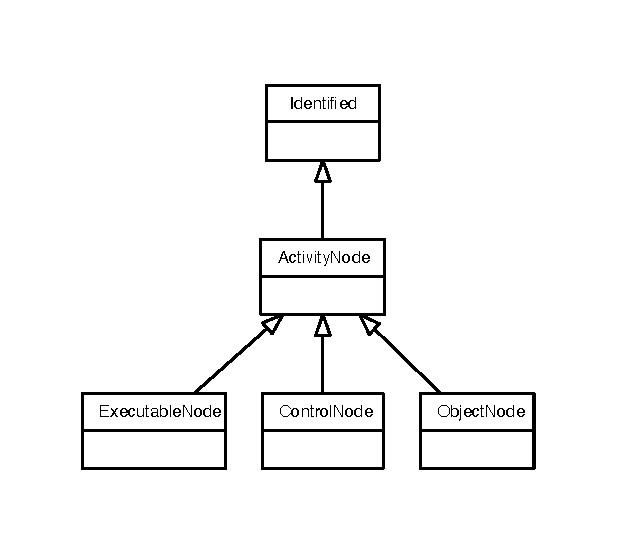
\includegraphics[width=1.0\textwidth]{uml_classes/ActivityNode_abstraction_hierarchy.pdf}%
\caption{ActivityNode}%
\label{fig:ActivityNode}%
\end{figure}

%
The \uml{ActivityNode} class is shown in \ref{fig:ActivityNode}. It is derived from \sbol{Identified} and includes the following specializations: \uml{ControlNode}, \uml{ObjectNode}, \uml{ExecutableNode}. %
%
\subsubsection{ControlNode}%
\label{sec:uml:ControlNode}%
A \uml{ControlNode} is a kind of \uml{ActivityNode} used to manage the flow of tokens between other nodes in an \prov{Activity}. It can manage branching and merging of workflows and the implementation of logic for flow control. See UML 2.5.1 specification section 15.3.%
\newline%
\linebreak%
The \uml{ControlNode} class is shown in \ref{fig:ActivityNode}. It is derived from \uml{ActivityNode} and includes the following specializations: \uml{InitialNode}, \uml{FinalNode}, \uml{ForkNode}, \uml{JoinNode}, \uml{MergeNode}, \uml{DecisionNode}. %
%
\paragraph{InitialNode}%
\label{sec:uml:InitialNode}%
An \uml{InitialNode} acts as a starting point for executing an \prov{Activity}. An \prov{Activity} may have more than \sbol{one} InitialNodes that start multiple concurrent control flows. See UML 2.5.1 specification section 15.3.%
\newline%
\linebreak%
The \uml{InitialNode} class is shown in \ref{fig:ActivityNode}. It is derived from \uml{ControlNode}.%
%
\paragraph{FinalNode}%
\label{sec:uml:FinalNode}%
A \uml{FinalNode} is a \uml{ControlNode} at which a flow in an \prov{Activity} stops. A \uml{FinalNode} shall not have outgoing ActivityEdges. See UML 2.5.1 specification section 15.3.%
\newline%
\linebreak%
The \uml{FinalNode} class is shown in \ref{fig:ActivityNode}. It is derived from \uml{ControlNode} and includes the following specializations: \uml{FlowFinalNode}. %
%
\subparagraph{FlowFinalNode}%
\label{sec:uml:FlowFinalNode}%
A \uml{FlowFinalNode} is a \uml{FinalNode} that terminates a flow. All tokens accepted by a \uml{FlowFinalNode} are destroyed. This has no effect on other flows in the \prov{Activity}. See UML 2.5.1 specification section 15.3.%
\newline%
\linebreak%
The \uml{FlowFinalNode} class is shown in \ref{fig:ActivityNode}. It is derived from \uml{FinalNode}.%
%
\paragraph{ForkNode}%
\label{sec:uml:ForkNode}%
A \uml{ForkNode} is a \uml{ControlNode} that splits a flow into multiple concurrent flows. A \uml{ForkNode} shall have exactly \sbol{one} incoming \uml{ActivityEdge}, though it may have multiple outgoing ActivityEdges. See UML 2.5.1 specification section 15.3.%
\newline%
\linebreak%
The \uml{ForkNode} class is shown in \ref{fig:ActivityNode}. It is derived from \uml{ControlNode}.%
%
\paragraph{JoinNode}%
\label{sec:uml:JoinNode}%
A \uml{JoinNode} is a \uml{ControlNode} that synchronizes multiple flows. A \uml{JoinNode} shall have exactly \sbol{one} outgoing \uml{ActivityEdge} but may have multiple incoming ActivityEdges. See UML 2.5.1 specification section 15.3.%
\newline%
\linebreak%
The \uml{JoinNode} class is shown in \ref{fig:ActivityNode}. It is derived from \uml{ControlNode}.%
%
\paragraph{MergeNode}%
\label{sec:uml:MergeNode}%
A \uml{MergeNode} is a control node that brings together multiple flows without synchronization. A \uml{MergeNode} shall have exactly \sbol{one} outgoing \uml{ActivityEdge} but may have multiple incoming ActivityEdges. See UML 2.5.1 specification section 15.3.%
\newline%
\linebreak%
The \uml{MergeNode} class is shown in \ref{fig:ActivityNode}. It is derived from \uml{ControlNode}.%
%
\paragraph{DecisionNode}%
\label{sec:uml:DecisionNode}%
A \uml{DecisionNode} is a \uml{ControlNode} that chooses between outgoing flows. A \uml{DecisionNode} shall have at least \sbol{one} and at most two incoming ActivityEdges, and at least \sbol{one} outgoing \uml{ActivityEdge}. See UML 2.5.1 specification section 15.3.%
\newline%
\linebreak%
The \uml{DecisionNode} class is shown in \ref{fig:ActivityNode}. It is derived from \uml{ControlNode}.%
This class includes the following properties: \uml{decisionInput}, \uml{decisionInputFlow}. %
\begin{itemize}%
\item%
The \uml{decisionInput} property is OPTIONAL and contains a URI reference to an associated object of type BehaviorA Behavior that is executed to provide an input to guard ValueSpecifications on ActivityEdges outgoing from the DecisionNode.%
\item%
The \uml{decisionInputFlow} property is OPTIONAL and contains a URI reference to an associated object of type ObjectFlowAn additional ActivityEdge incoming to the DecisionNode that provides a decision input value for the guards ValueSpecifications on ActivityEdges outgoing from the DecisionNode.%
\end{itemize}%
\subsubsection{ObjectNode}%
\label{sec:uml:ObjectNode}%
An \uml{ObjectNode} is a kind of \uml{ActivityNode} used to hold value-containing object tokens during the course of the execution of an \prov{Activity}. See UML 2.5.1 specification section 15.4.%
\newline%
\linebreak%
The \uml{ObjectNode} class is shown in \ref{fig:ActivityNode}. It is derived from \uml{ActivityNode} and includes the following specializations: \uml{ActivityParameterNode}, \uml{Pin}. %
This class includes the following properties: \uml{type}. %
\begin{itemize}%
\item%
The \uml{type} property is OPTIONAL and has a singleton value of type URISpecifies a set of Type instances constraining the allowed values. See UML 2.5.1 specification section 7.5.%
\end{itemize}%
\paragraph{ActivityParameterNode}%
\label{sec:uml:ActivityParameterNode}%
An \uml{ActivityParameterNode} is an \uml{ObjectNode} for accepting values from the input Parameters or providing values to the output Parameters of an \prov{Activity}. UML 2.5.1 specification section 15.4.%
\newline%
\linebreak%
The \uml{ActivityParameterNode} class is shown in \ref{fig:ActivityNode}. It is derived from \uml{ObjectNode}.%
This class includes the following properties: \uml{parameter}. %
\begin{itemize}%
\item%
The \uml{parameter} property is REQUIRED and contains a URI reference to an associated object of type ParameterThe Parameter for which the ActivityParameterNode will be accepting or providing values.%
\end{itemize}%
\paragraph{Pin}%
\label{sec:uml:Pin}%
A \uml{Pin} is an \uml{ObjectNode} and MultiplicityElement that provides input values to an \uml{Action} or accepts output values from an \uml{Action}. See UML 2.5.1 specification section 16.2.%
\newline%
\linebreak%
The \uml{Pin} class is shown in \ref{fig:ActivityNode}. It is derived from \uml{ObjectNode} and includes the following specializations: \uml{InputPin}, \uml{OutputPin}. %
This class includes the following properties: \uml{isOrdered}, \uml{isUnique}, \uml{upperValue}, \uml{lowerValue}. %
\begin{itemize}%
\item%
The \uml{upperValue} property is OPTIONAL and contains a URI reference to an associated object of type ValueSpecificationFor MultiplicityElement abstract class; UML 2.5.1 specification section 7.5%
\item%
The \uml{lowerValue} property is OPTIONAL and contains a URI reference to an associated object of type ValueSpecificationFor MultiplicityElement abstract class; UML 2.5.1 specification section 7.5%
\item%
The \uml{isOrdered} property is REQUIRED and has a singleton value of type booleanFor MultiplicityElement abstract class; UML 2.5.1 specification section 7.5%
\item%
The \uml{isUnique} property is REQUIRED and has a singleton value of type booleanFor MultiplicityElement abstract class; UML 2.5.1 specification section 7.5%
\end{itemize}%
\subparagraph{InputPin}%
\label{sec:uml:InputPin}%
An \uml{InputPin} is a \uml{Pin} that holds input values to be consumed by an \uml{Action}. See UML 2.5.1 specification section 16.2.%
\newline%
\linebreak%
The \uml{InputPin} class is shown in \ref{fig:ActivityNode}. It is derived from \uml{Pin} and includes the following specializations: \uml{ValuePin}. %
%
\subparagraph{ValuePin}%
\label{sec:uml:ValuePin}%
A \uml{ValuePin} is an \uml{InputPin} that provides a value by evaluating a \uml{ValueSpecification}. See UML 2.5.1 specification section 16.2.%
\newline%
\linebreak%
The \uml{ValuePin} class is shown in \ref{fig:ActivityNode}. It is derived from \uml{InputPin}.%
This class includes the following properties: \uml{value}. %
\begin{itemize}%
\item%
The \uml{value} property is REQUIRED and contains a URI reference to an associated object of type ValueSpecificationThe ValueSpecification that is evaluated to obtain the value that the ValuePin will provide.%
\end{itemize}%
\subparagraph{OutputPin}%
\label{sec:uml:OutputPin}%
An \uml{OutputPin} is a \uml{Pin} that holds output values produced by an \uml{Action}. See UML 2.5.1 specification section 16.2.%
\newline%
\linebreak%
The \uml{OutputPin} class is shown in \ref{fig:ActivityNode}. It is derived from \uml{Pin}.%
%
\subsubsection{ExecutableNode}%
\label{sec:uml:ExecutableNode}%
An \uml{ExecutableNode} is an abstract class for ActivityNodes whose execution may be controlled using ControlFlows and to which ExceptionHandlers may be attached. See UML 2.5.1 specification section 15.5.%
\newline%
\linebreak%
The \uml{ExecutableNode} class is shown in \ref{fig:ActivityNode}. It is derived from \uml{ActivityNode} and includes the following specializations: \uml{Action}. %
%
\paragraph{Action}%
\label{sec:uml:Action}%
An \uml{Action} is the fundamental unit of executable functionality. The execution of an \uml{Action} represents some transformation or processing in the modeled system. Actions provide the ExecutableNodes within Activities and may also be used within Interactions. See UML 2.5.1 specification section 16.%
\newline%
\linebreak%
The \uml{Action} class is shown in \ref{fig:ActivityNode}. It is derived from \uml{ExecutableNode} and includes the following specializations: \uml{InvocationAction}. %
This class includes the following properties: \uml{output}, \uml{input}. %
\begin{itemize}%
\item%
The \uml{output} property is OPTIONAL and contains URI references to associated objects of type OutputPinThe ordered set of OutputPins representing outputs from the Action.%
\item%
The \uml{input} property is OPTIONAL and contains URI references to associated objects of type InputPinThe ordered set of InputPins representing the inputs to the Action.%
\end{itemize}%
\subparagraph{InvocationAction}%
\label{sec:uml:InvocationAction}%
UML 2.5.1 specification section 16.3%
\newline%
\linebreak%
The \uml{InvocationAction} class is shown in \ref{fig:ActivityNode}. It is derived from \uml{Action} and includes the following specializations: \uml{CallAction}. %
%
\subparagraph{CallAction}%
\label{sec:uml:CallAction}%
A \uml{CallAction} is an abstract class for Actions that invoke a \uml{Behavior} with given argument values and (if the invocation is synchronous) receive reply values. See UML 2.5.1 specification section 16.3.%
\newline%
\linebreak%
The \uml{CallAction} class is shown in \ref{fig:ActivityNode}. It is derived from \uml{InvocationAction} and includes the following specializations: \uml{CallBehaviorAction}. %
%
\subparagraph{CallBehaviorAction}%
\label{sec:uml:CallBehaviorAction}%
A \uml{CallBehaviorAction} is a \uml{CallAction} that invokes a \uml{Behavior} directly. The argument values of the \uml{CallBehaviorAction} are passed on the input Parameters of the invoked \uml{Behavior}. UML 2.5.1 specification section 16.3%
\newline%
\linebreak%
The \uml{CallBehaviorAction} class is shown in \ref{fig:ActivityNode}. It is derived from \uml{CallAction}.%
This class includes the following properties: \uml{behavior}. %
\begin{itemize}%
\item%
The \uml{behavior} property is REQUIRED and contains a URI reference to an associated object of type BehaviorThe Behavior being invoked.%
\end{itemize}%
\subsection{ActivityEdge}%
\label{sec:uml:ActivityEdge}%
An \uml{ActivityEdge} is an abstract class for directed connections between two ActivityNodes. See UML 2.5.1 specification section 15.2.%
\newline%
\linebreak%


\begin{figure}[h!]%
\centering%
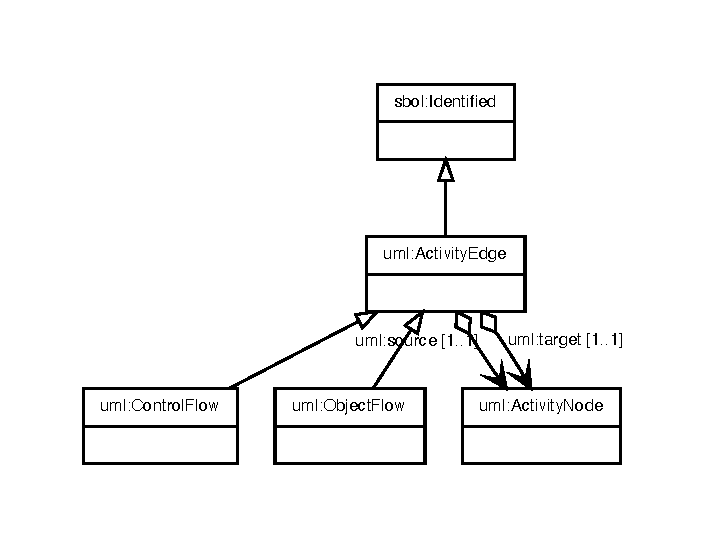
\includegraphics[width=0.5063829787234042\textwidth]{uml_classes/ActivityEdge_abstraction_hierarchy.pdf}%
\caption{ActivityEdge}%
\label{fig:ActivityEdge}%
\end{figure}

%
The \uml{ActivityEdge} class is shown in \ref{fig:ActivityEdge}. It is derived from \sbol{Identified} and includes the following specializations: \uml{ControlFlow}, \uml{ObjectFlow}. %
This class includes the following properties: \uml{source}, \uml{target}. %
\begin{itemize}%
\item%
The \uml{source} property is REQUIRED and contains a URI reference to an associated object of type ActivityNodeThe ActivityNode from which tokens are taken when they traverse the ActivityEdge.%
\item%
The \uml{target} property is REQUIRED and contains a URI reference to an associated object of type ActivityNodeThe ActivityNode to which tokens are put when they traverse the ActivityEdge.%
\end{itemize}%
\subsubsection{ControlFlow}%
\label{sec:uml:ControlFlow}%
A \uml{ControlFlow} is an \uml{ActivityEdge} traversed by control tokens or object tokens of control type, which are use to control the execution of ExecutableNodes. See UML 2.5.1 specification section 15.2.%
\newline%
\linebreak%
The \uml{ControlFlow} class is shown in \ref{fig:ActivityEdge}. It is derived from \uml{ActivityEdge}.%
%
\subsubsection{ObjectFlow}%
\label{sec:uml:ObjectFlow}%
An \uml{ObjectFlow} is an \uml{ActivityEdge} that is traversed by object tokens that may hold values. Object flows also support multicast/receive, token selection from object nodes, and transformation of tokens. See UML 2.5.1 specification section 15.2.%
\newline%
\linebreak%
The \uml{ObjectFlow} class is shown in \ref{fig:ActivityEdge}. It is derived from \uml{ActivityEdge}.%
%
